\documentclass[12pt, a4paper]{book}

\usepackage[T1]{fontenc}
\usepackage[utf8]{inputenc}
\usepackage[charter, cal=cmcal]{mathdesign}
\usepackage[scaled=0.92]{helvet}
\usepackage{geometry}
\geometry{a4paper, top=30mm, bottom=30mm, inner=32mm, outer=25mm, marginparwidth=18mm}

\usepackage{amsmath, amsthm}
\usepackage[version=4]{mhchem}
\usepackage{graphicx}
\usepackage{xcolor}
\usepackage{tikz}
\usetikzlibrary{arrows.meta, shapes.geometric, positioning, calc, backgrounds}
\usepackage{pgfplots}
\pgfplotsset{compat=1.18}
\usepackage{tcolorbox}
\tcbuselibrary{skins, breakable, theorems}
\usepackage{titlesec}
\usepackage{fancyhdr}
\usepackage{enumitem}
\usepackage{booktabs}
\usepackage{array}
\usepackage{parskip}
\usepackage{siunitx}
\usepackage[colorlinks=true, linkcolor=BrickRed,
            urlcolor=NavyBlue, citecolor=ForestGreen]{hyperref}

% ── Colours (Journey 8 — forest green / amber) ────────────────────────────────
\definecolor{JourneyColor}{HTML}{065F46}
\definecolor{ModuleColor}{HTML}{059669}
\definecolor{PuzzleColor}{HTML}{B45309}
\definecolor{DiscoveryColor}{HTML}{D97706}
\definecolor{WarningColor}{HTML}{991B1B}
\definecolor{ProblemColor}{HTML}{6B21A8}
\definecolor{ReflectColor}{HTML}{0D9488}
\definecolor{HistoryColor}{HTML}{78350F}

% ── Boxes ─────────────────────────────────────────────────────────────────────
\newtcolorbox{puzzlebox}[1][]{enhanced,breakable,
  colback=PuzzleColor!6,colframe=PuzzleColor,fonttitle=\bfseries\sffamily,
  title={The Puzzle},attach boxed title to top left={yshift=-2mm,xshift=6mm},
  boxed title style={colback=PuzzleColor},borderline west={3pt}{0pt}{PuzzleColor},#1}

\newtcolorbox{discoverybox}[1][]{enhanced,breakable,
  colback=DiscoveryColor!8,colframe=DiscoveryColor,fonttitle=\bfseries\sffamily,
  title={Discovery},attach boxed title to top left={yshift=-2mm,xshift=6mm},
  boxed title style={colback=DiscoveryColor},borderline west={3pt}{0pt}{DiscoveryColor},#1}

\newtcolorbox{problembox}[1][]{enhanced,breakable,
  colback=ProblemColor!5,colframe=ProblemColor,fonttitle=\bfseries\sffamily,
  title={Problems},attach boxed title to top left={yshift=-2mm,xshift=6mm},
  boxed title style={colback=ProblemColor},borderline west={3pt}{0pt}{ProblemColor},#1}

\newtcolorbox{deepbox}[1][]{enhanced,breakable,
  colback=JourneyColor!5,colframe=JourneyColor,fonttitle=\bfseries\sffamily,
  title={Deep Problems},attach boxed title to top left={yshift=-2mm,xshift=6mm},
  boxed title style={colback=JourneyColor},borderline west={4pt}{0pt}{JourneyColor},#1}

\newtcolorbox{historybox}[1][]{enhanced,breakable,
  colback=HistoryColor!7,colframe=HistoryColor!60,fonttitle=\bfseries\sffamily\small,
  title={Historical Note},attach boxed title to top left={yshift=-2mm,xshift=6mm},
  boxed title style={colback=HistoryColor!80},#1}

\newtcolorbox{reflectionbox}[1][]{enhanced,breakable,
  colback=ReflectColor!6,colframe=ReflectColor,fonttitle=\bfseries\sffamily,
  title={Reflection},attach boxed title to top left={yshift=-2mm,xshift=6mm},
  boxed title style={colback=ReflectColor},borderline west={3pt}{0pt}{ReflectColor},#1}

\newtcolorbox{namedconcept}[2][]{enhanced,
  colback=ModuleColor!6,colframe=ModuleColor,fonttitle=\bfseries\sffamily\large,
  title={#2},attach boxed title to top left={yshift=-2mm,xshift=6mm},
  boxed title style={colback=ModuleColor},#1}

% ── Section formatting ────────────────────────────────────────────────────────
\titleformat{\chapter}[display]
  {\normalfont\sffamily\huge\bfseries\color{JourneyColor}}
  {\textcolor{JourneyColor!60}{\chaptertitlename\ \thechapter}}{10pt}{\Huge}
  [\vspace{2pt}\textcolor{JourneyColor}{\titlerule[1.5pt]}]
\titleformat{\section}
  {\normalfont\sffamily\Large\bfseries\color{ModuleColor}}
  {\thesection}{1em}{}[\textcolor{ModuleColor!40}{\titlerule[0.6pt]}]
\titleformat{\subsection}
  {\normalfont\sffamily\large\bfseries\color{JourneyColor!80}}{\thesubsection}{1em}{}
\titleformat{\subsubsection}
  {\normalfont\sffamily\normalsize\bfseries}{\thesubsubsection}{1em}{}

\pagestyle{fancy}
\fancyhf{}
\fancyhead[LE]{\small\sffamily\textcolor{JourneyColor}{\leftmark}}
\fancyhead[RO]{\small\sffamily\textcolor{ModuleColor}{\rightmark}}
\fancyfoot[C]{\small\thepage}
\renewcommand{\headrulewidth}{0.4pt}

\newcommand{\newterm}[1]{\textit{\textcolor{DiscoveryColor}{#1}}}
\newcommand{\important}[1]{\textcolor{ModuleColor}{\textbf{#1}}}

\begin{document}

\setcounter{chapter}{7}
\setcounter{section}{1}

\section{Module 8.2 --- Silicon Doping and Semiconductors}

Pure silicon is a poor conductor at room temperature. Its band gap of \SI{1.12}{eV} is large enough that only a tiny fraction of electrons are thermally promoted to the conduction band. However, by substituting a minute fraction of silicon atoms with elements from Group 13 or Group 15, we can modify its electronic structure. This process is called doping.

\newpage

% ─── Section: The Puzzle ─────────────────────────────────────────────────────
\section{Part 1 --- The Puzzle}

\begin{puzzlebox}
\textbf{The Boundary Potential of Junctions}

Suppose we join a piece of silicon doped with phosphorus (n-type) to a piece doped with boron (p-type) to form a single continuous crystal interface (a p-n junction).

\medskip
\begin{center}
\begin{tikzpicture}[scale=0.8]
  \draw[fill=blue!10, draw=JourneyColor, thick] (0,0) rect (4,2.5);
  \draw[fill=red!10, draw=JourneyColor, thick] (4,0) rect (8,2.5);
  \node at (2,1.25) {\large\bfseries p-type};
  \node at (6,1.25) {\large\bfseries n-type};
  \draw[line width=1.5pt, teal] (4,-0.2) -- (4,2.7) node[above] {Junction};
\end{tikzpicture}
\end{center}

\medskip
\textbf{Question 1.} In the n-type region, there is a high concentration of free electrons. In the p-type region, there is a high concentration of holes (electron vacancies). What thermodynamic driving force governs the behavior of these carriers immediately after the junction is created?

\textbf{Question 2.} As electrons diffuse from the n-type side into the p-type side and holes diffuse from the p-type side into the n-type side, they recombine and annihilate. What remains behind near the junction boundary on each side? What charge do these remaining dopant ions carry?

\textbf{Question 3.} Draw the resulting electric field vector at the junction interface. Does this field encourage or oppose further diffusion of carriers? How does the system reach equilibrium?
\end{puzzlebox}

\newpage

% ─── Section: Exploration ────────────────────────────────────────────────────
\section{Part 2 --- Exploration}

\subsection{Step 1: Carrier Densities and the Fermi Level}

\begin{problembox}
The concentration of electrons $n$ in the conduction band and holes $p$ in the valence band at thermal equilibrium are given by:
\[
  n \;=\; N_C e^{-\frac{E_C - E_F}{k_B T}}, \quad p \;=\; N_V e^{-\frac{E_F - E_V}{k_B T}},
\]
where $E_C$ is the conduction band edge, $E_V$ is the valence band edge, $E_F$ is the Fermi level, and $N_C, N_V$ are the effective densities of states.

\begin{enumerate}[label=(\alph*)]
  \item Show that the product of the electron and hole concentrations is independent of the Fermi level and is given by the law of mass action:
        \[
          np \;=\; n_i^2 \;=\; N_C N_V e^{-\frac{E_g}{k_B T}},
        \]
        where $E_g = E_C - E_V$ is the band gap.
  \item In intrinsic (pure) silicon, $n = p = n_i$. For silicon at room temperature ($T = \SI{300}{K}$), $n_i \approx \SI{1.5e10}{cm^{-3}}$. Calculate $n$ and $p$ if we substitute silicon atoms to introduce a donor concentration of $N_D = \SI{1.0e16}{cm^{-3}}$ (assume all donors are ionized so $n \approx N_D$).
  \item Explain why the minority carrier concentration (holes in n-type silicon) drops drastically compared to its value in pure silicon. Where did they go?
\end{enumerate}
\end{problembox}

\subsection{Step 2: The Depletion Approximation and Poisson's Equation}

\begin{problembox}
Across a p-n junction, the diffusion of carriers leaves a region devoid of mobile charges. This is called the \newterm{depletion region}.
Let the depletion region extend a distance $x_p$ into the p-type side and $x_n$ into the n-type side, with doping concentrations $N_A$ (acceptors) and $N_D$ (donors).

\begin{enumerate}[label=(\alph*)]
  \item By charge neutrality, the total negative charge on the p-side must equal the total positive charge on the n-side. Write this relation in terms of $N_A, N_D, x_p,$ and $x_n$.
  \item In the depletion region ($-x_p \le x \le x_n$), the charge density $\rho(x)$ is:
        \[
          \rho(x) \;=\; \begin{cases}
            -q N_A & \text{for } -x_p \le x < 0, \\
            q N_D  & \text{for } 0 < x \le x_n.
          \end{cases}
        \]
        Using Poisson's equation $\frac{d^2 V}{dx^2} = -\frac{\rho}{\varepsilon}$, integrate twice to find the electric field $E(x) = -\frac{dV}{dx}$ and the potential $V(x)$ in both regions, assuming $E(-x_p) = E(x_n) = 0$ and $V(-x_p) = 0$.
\end{enumerate}
\end{problembox}

\newpage

% ─── Section: Discovery ──────────────────────────────────────────────────────
\section{Part 3 --- Discovery}

\begin{discoverybox}
\textbf{The Built-in Potential}

The Fermi level must be constant throughout a system at thermodynamic equilibrium. Because the Fermi level lies close to the conduction band in n-type silicon and close to the valence band in p-type silicon, joining them forces the bands to bend. This bending creates a potential barrier $V_{bi}$, the \newterm{built-in potential}.

\begin{center}
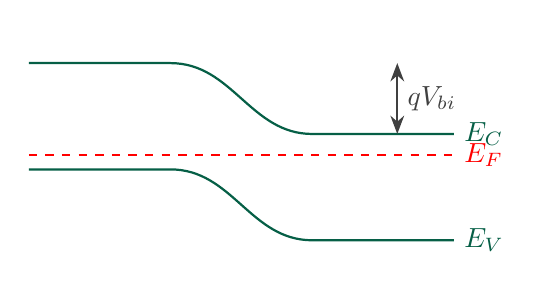
\begin{tikzpicture}[scale=0.9]
  \draw[thick, JourneyColor] (0,2.5) -- (2,2.5) to[out=0,in=180] (4,1.5) -- (6,1.5) node[right] {$E_C$};
  \draw[thick, JourneyColor] (0,1.0) -- (2,1.0) to[out=0,in=180] (4,0.0) -- (6,0.0) node[right] {$E_V$};
  \draw[dashed, red, thick] (0,1.2) -- (6,1.2) node[right] {$E_F$};
  
  \draw[<->, >=Stealth, thick, darkgray] (5.2, 1.5) -- (5.2, 2.5) node[midway, right] {$q V_{bi}$};
  \draw[draw=none] (2,-0.5) -- (2,3.0);
\end{tikzpicture}
\end{center}

By equating the drift and diffusion currents of carriers at equilibrium, we find:
\[
  V_{bi} \;=\; \frac{k_B T}{q} \ln\left(\frac{N_A N_D}{n_i^2}\right).
\]
This potential difference is not measurable with a standard voltmeter because contact potentials at the metal-semiconductor probes exactly cancel it. However, it sets the threshold for carrier injection under external bias.
\end{discoverybox}

\newpage

% ─── Section: What This Is Called ────────────────────────────────────────────
\section{Part 4 --- What This Is Called}

\begin{namedconcept}{Extrinsic Semiconductors}
\begin{itemize}
  \item \important{Donor:} An impurity atom with more valence electrons than the host crystal (e.g., Phosphorus in Silicon). It donates an electron to the conduction band, leaving a fixed positive ion ($N_D^+$).
  \item \important{Acceptor:} An impurity atom with fewer valence electrons than the host crystal (e.g., Boron in Silicon). It accepts an electron from the valence band, generating a hole and leaving a fixed negative ion ($N_A^-$).
  \item \important{n-type Semiconductor:} A semiconductor where electrons are the majority carriers ($n \gg p$).
  \item \important{p-type Semiconductor:} A semiconductor where holes are the majority carriers ($p \gg n$).
  \item \important{Built-in Potential ($V_{bi}$):} The electrostatic potential barrier established across a p-n junction at equilibrium due to carrier diffusion.
\end{itemize}
\end{namedconcept}

\newpage

% ─── Section: Solved Exercises ───────────────────────────────────────────────
\section{Part 5 --- Solved Exercises}

\begin{problembox}
\textbf{Exercise:} A silicon p-n junction at $T = \SI{300}{K}$ has $N_A = \SI{2.0e16}{cm^{-3}}$ and $N_D = \SI{1.0e15}{cm^{-3}}$. The dielectric permittivity of silicon is $\varepsilon = 11.7\,\varepsilon_0 \approx \SI{1.04e-12}{F/cm}$.
\begin{enumerate}
  \item Calculate the built-in potential $V_{bi}$.
  \item Find the total depletion width $W = x_n + x_p$ using the formula:
        \[
          W \;=\; \sqrt{\frac{2\varepsilon V_{bi}}{q}\left(\frac{1}{N_A} + \frac{1}{N_D}\right)}.
        \]
\end{enumerate}

\textbf{Solution:}
\begin{enumerate}
  \item Using the formula for $V_{bi}$:
        \[
          V_{bi} \;=\; \frac{k_B T}{q} \ln\left(\frac{N_A N_D}{n_i^2}\right).
        \]
        At $T = \SI{300}{K}$, $\frac{k_B T}{q} \approx \SI{0.0259}{V}$, and $n_i \approx \SI{1.5e10}{cm^{-3}}$.
        \[
          V_{bi} \;=\; 0.0259 \ln\left(\frac{2.0e16 \times 1.0e15}{(1.5e10)^2}\right) \;\approx\; 0.0259 \ln\left(\frac{2.0e31}{2.25e20}\right) \;\approx\; \SI{0.655}{V}.
        \]
  \item Substitute the values into the depletion width formula ($q = \SI{1.602e-19}{C}$):
        \[
          \frac{1}{N_A} + \frac{1}{N_D} \;=\; \frac{1}{2.0e16} + \frac{1}{1.0e15} \;=\; 5.0e-17 + 1.0e-15 \;=\; \SI{1.05e-15}{cm^3}.
        \]
        \[
          W \;=\; \sqrt{\frac{2 \times 1.04e-12 \times 0.655}{1.602e-19} \times 1.05e-15} \;\approx\; \sqrt{8.50e-9 \times 1.05e-15} \;\approx\; \SI{9.45e-5}{cm} \;=\; \SI{0.945}{\mu m}.
        \]
\end{enumerate}
\end{problembox}

\newpage

% ─── Section: Problems ───────────────────────────────────────────────────────
\section{Part 6 --- Problems}

\begin{problembox}
\begin{enumerate}[label=\textbf{P\arabic*.}]
  \item \textbf{Fermi Level Shift in n-type Silicon.}
  
        For a silicon sample doped with phosphorus at $N_D = \SI{5.0e17}{cm^{-3}}$, calculate:
        \begin{enumerate}[label=(\alph*)]
          \item The position of the Fermi level $E_F$ relative to the intrinsic Fermi level $E_i \approx (E_C+E_V)/2$ at $T = \SI{300}{K}$ (use $E_F - E_i = k_B T \ln(n/n_i)$).
          \item How this difference $E_F - E_i$ changes if the sample is heated to $T = \SI{450}{K}$. (Note: $n_i(T)$ increases rapidly with temperature).
        \end{enumerate}

  \item \textbf{Reverse and Forward Bias Band Diagrams.}
  
        When an external voltage $V_a$ is applied across the junction, the potential barrier becomes $V_{bi} - V_a$.
        \begin{enumerate}[label=(\alph*)]
          \item Draw the band diagrams under forward bias ($V_a > 0$) and reverse bias ($V_a < 0$).
          \item Explain how these biases modulate the depletion width $W$ and the current flowing through the device.
        \end{enumerate}
\end{enumerate}
\end{problembox}

\newpage

% ─── Section: Deep Problems ──────────────────────────────────────────────────
\section{Part 7 --- Deep Problems}

\begin{deepbox}
\begin{enumerate}[label=\textbf{D\arabic*.}]
  \item \textbf{Derivation of the Ideal Diode Equation.}
  
        The current in a p-n junction under bias $V_a$ is dominated by diffusion of minority carriers injected across the depletion region boundary.
        Let $p_n(x)$ be the hole concentration in the n-type region ($x > x_n$). The steady-state diffusion equation for holes is:
        \[
          D_p \frac{d^2 p_n}{dx^2} - \frac{p_n - p_{n0}}{\tau_p} \;=\; 0,
        \]
        where $D_p$ is the hole diffusion coefficient, $\tau_p$ is the hole lifetime, and $p_{n0} = n_i^2/N_D$ is the equilibrium hole concentration.
        \begin{enumerate}[label=(\alph*)]
          \item Solve this differential equation subject to the boundary conditions:
                * $p_n(x_n) = p_{n0} e^{\frac{q V_a}{k_B T}}$ (minority injection at boundary)
                * $p_n(x \to \infty) = p_{n0}$ (recombination back to equilibrium)
          \item Calculate the hole diffusion current density $J_p = -q D_p \frac{dp_n}{dx}\Big|_{x_n}$.
          \item By adding the analogous electron current density $J_n$ from the p-side, prove the Shockley ideal diode equation:
                \[
                  J \;=\; J_0 \left(e^{\frac{q V_a}{k_B T}} - 1\right),
                \]
                and express the reverse saturation current density $J_0$ in terms of $D_p, D_n, \tau_p, \tau_n, N_A, N_D,$ and $n_i$.
        \end{enumerate}
\end{enumerate}
\end{deepbox}

\newpage

% ─── Section: Reflection ─────────────────────────────────────────────────────
\section{Part 8 --- Reflection}

\begin{reflectionbox}
\textbf{Conceptual Reflection}

\begin{enumerate}
  \item **Entropy vs. Electrostatics:** The formation of the depletion region is a competition between the entropy of mixing (carriers want to diffuse to maximize configuration entropy) and electrostatic energy (attraction of remaining ions). Discuss how this balance illustrates the second law of thermodynamics.
  \item **The Scale of Control:** In modern integrated circuits, silicon channels are doped with just a few thousand dopant atoms. At these nanoscale dimensions, statistical fluctuations in the number of dopant atoms lead to device-to-device variability. What does this reveal about the limits of deterministic solid-state scaling?
\end{enumerate}
\end{reflectionbox}

\vspace{1.4cm}
\begin{center}
{\color{JourneyColor}\rule{0.5\linewidth}{0.8pt}}\\[6pt]
{\small\color{JourneyColor}\textit{End of Journey 8, Module 8.2 --- Silicon Doping and Semiconductors}}\\[4pt]
{\small\color{JourneyColor}Continue to: \textbf{Module 8.3 --- Metals, Alloys, and Mechanical Properties}}\\[6pt]
{\color{JourneyColor}\rule{0.5\linewidth}{0.8pt}}
\end{center}

\end{document}
